\documentclass[10pt]{article}

\usepackage[utf8]{inputenc}
\usepackage[spanish]{babel}
\decimalpoint
\usepackage{amsmath, amssymb}
\usepackage{xcolor}
\usepackage{geometry}
\geometry{letterpaper, margin=1in}
\usepackage{graphicx}
\usepackage{hyperref}
\usepackage{float}
\usepackage{colortbl}
\usepackage{caption}


\title{Universidad Panamericana \\ Maestría en Ciencia de Datos \\ Econometría \\ \vspace{0.5cm} Actividad RLS}
\author{Enrique Ulises Báez Gómez Tagle}
\date{\today}

\begin{document}

\maketitle

\tableofcontents

\newpage

\section{Ejercicio 1}
	Se realizó un estudio para determinar si ciertas medidas de la fuerza estática del brazo influyen en las características de ``levantamiento dinámico'' de un individuo. Veinticinco individuos se sometieron a pruebas de fuerza y luego se les pidió que hicieran una prueba de levantamiento de peso, en el que el peso se elevaba en forma dinámica por encima de la cabeza. A continuación se presentan los datos.

	\begin{table}[H]
		\centering
		\caption{Datos de fuerza del brazo y levantamiento dinámico}
		\label{tab:datos_fuerza}
		\begin{tabular}{|c|c|c|}
			\hline
			\textbf{Individuo} & \textbf{Fuerza del brazo, $x$} & \textbf{Levantamiento dinámico, $y$} \\
			\hline
			1  & 17.3 & 71.7 \\
			2  & 19.3 & 48.3 \\
			3  & 19.5 & 88.3 \\
			4  & 19.7 & 75.0 \\
			5  & 22.9 & 91.7 \\
			6  & 23.1 & 100.0 \\
			7  & 26.4 & 73.3 \\
			8  & 26.8 & 65.0 \\
			9  & 27.6 & 75.0 \\
			10 & 28.1 & 88.3 \\
			11 & 28.2 & 68.3 \\
			12 & 28.7 & 96.7 \\
			13 & 29.0 & 76.7 \\
			14 & 29.6 & 78.3 \\
			15 & 29.9 & 60.0 \\
			16 & 29.9 & 71.7 \\
			17 & 30.3 & 85.0 \\
			18 & 31.3 & 85.0 \\
			19 & 36.0 & 88.3 \\
			20 & 39.5 & 100.0 \\
			21 & 40.4 & 100.0 \\
			22 & 44.3 & 100.0 \\
			23 & 44.6 & 91.7 \\
			24 & 50.4 & 100.0 \\
			25 & 55.9 & 71.7 \\
			\hline
		\end{tabular}
	\end{table}

	\begin{itemize}
		\item \textbf{a.} Realice el diagrama de dispersión entre las variables, obtenga e interpreta las estadísticas descriptivas de las mismas.\\
		\textcolor{blue}{El diagrama de dispersión muestra una tendencia positiva moderada entre la fuerza del brazo ($x$) y el levantamiento dinámico ($y$). Al analizar las estadísticas descriptivas, se observa que ambas variables presentan medias cercanas a sus medianas, lo que indica una distribución relativamente simétrica.\\
		\begin{figure}[H]
			\centering
			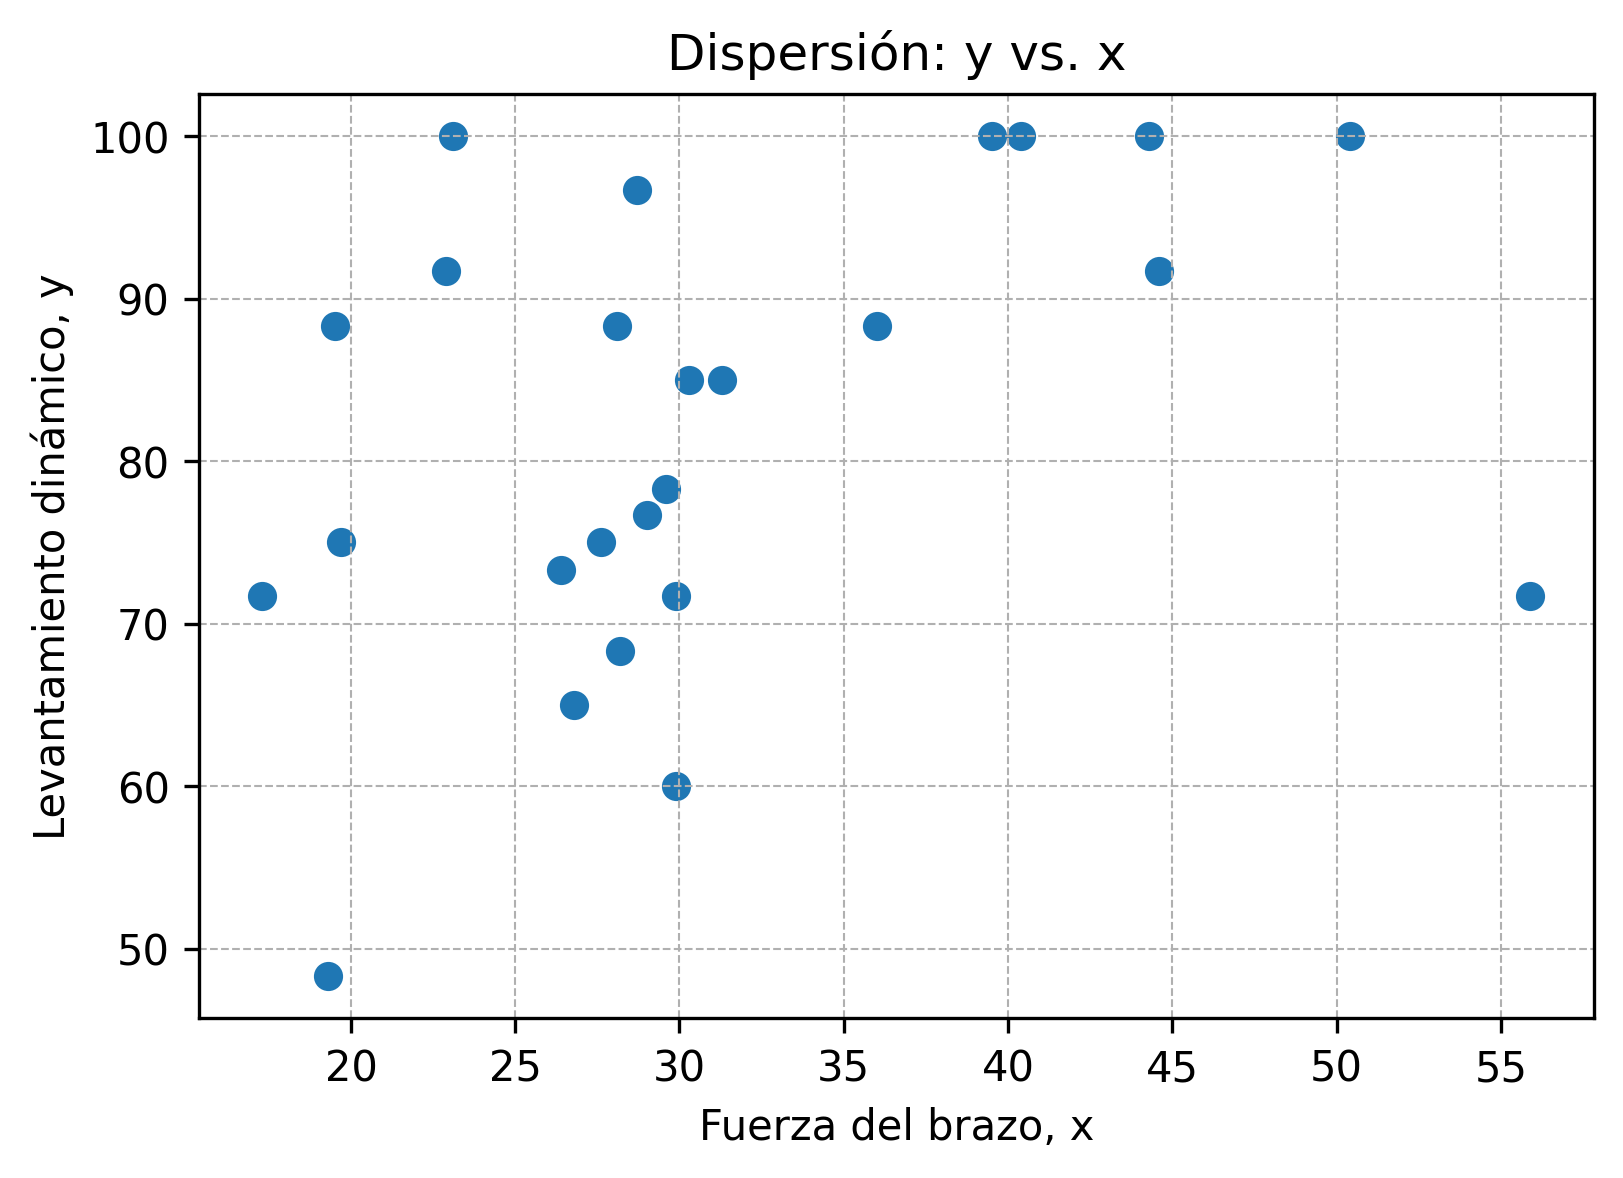
\includegraphics[width=0.7\textwidth]{../plots/python/ejercicio1/scatter_plot.png}
			\caption{Dispersión: $y$ vs. $x$.}
			\label{fig:scatter}
		\end{figure}
			\noindent\textbf{Estadísticas descriptivas}
			\begin{center}
				\begin{tabular}{lccccccc}
					\hline
					Variable & Media & Mediana & Desv. Est. & Min & Q1 & Q3 & Max \\
					\hline
					Fuerza del brazo $x$ & 31.15 & 29.0 & 9.87 & 17.3 & 26.4 & 36.0 & 55.9 \\
					Levantamiento dinámico $y$ & 82.00 & 85.0 & 14.13 & 48.3 & 71.7 & 91.7 & 100.0 \\
					\hline
				\end{tabular}
			\end{center}
		}

		\item \textbf{b.} Calcule el coeficiente de correlación lineal y realice la prueba de hipótesis correspondiente para validar si existe o no relación lineal entre las variables, con una significancia del 5\%.\\
		\textcolor{blue}{
			El coeficiente de Pearson es
			\[
				r=0.3917, \quad p\text{-valor}=0.0528.
			\]
			Con $p>\alpha=0.05$ no se rechaza $H_0: \rho=0$; no hay evidencia suficiente de relación lineal al 5\%.
		}
		

		\item \textbf{c.} Estime los coeficientes del modelo de regresión lineal simple por MCO.\\
		\textcolor{blue}{
			El modelo estimado es: \[
			\hat{y}=64.53+0.561\,x, \qquad R^2=0.153.
			\]
			La pendiente es marginalmente no significativa ($p=0.053$), mientras que el intercepto sí lo es ($p<0.01$).
		}


		\item \textbf{d.} Obtenga la estimación puntual para una fuerza del brazo de 30.\\
		\textcolor{blue}{		
			\[
				\hat{y}\,(30)=81.36,
			\]
			IC del 95\% para la media condicional: $[75.82,\,86.89]$; intervalo de predicción del 95\%: $[53.33,\,109.38]$.	
		}

		\item \textbf{e.} Grafique los residuales en comparación con la variable independiente y comente los resultados.\\
		\textcolor{blue}{
			La Figura~\ref{fig:resid} muestra residuales centrados en cero ($\bar e\approx0$) y prácticamente incorrelacionados con $x$ (\(\mathrm{corr}(x,e)\approx0\)), consistente con los supuestos de MCO.
			\begin{figure}[H]
				\centering
				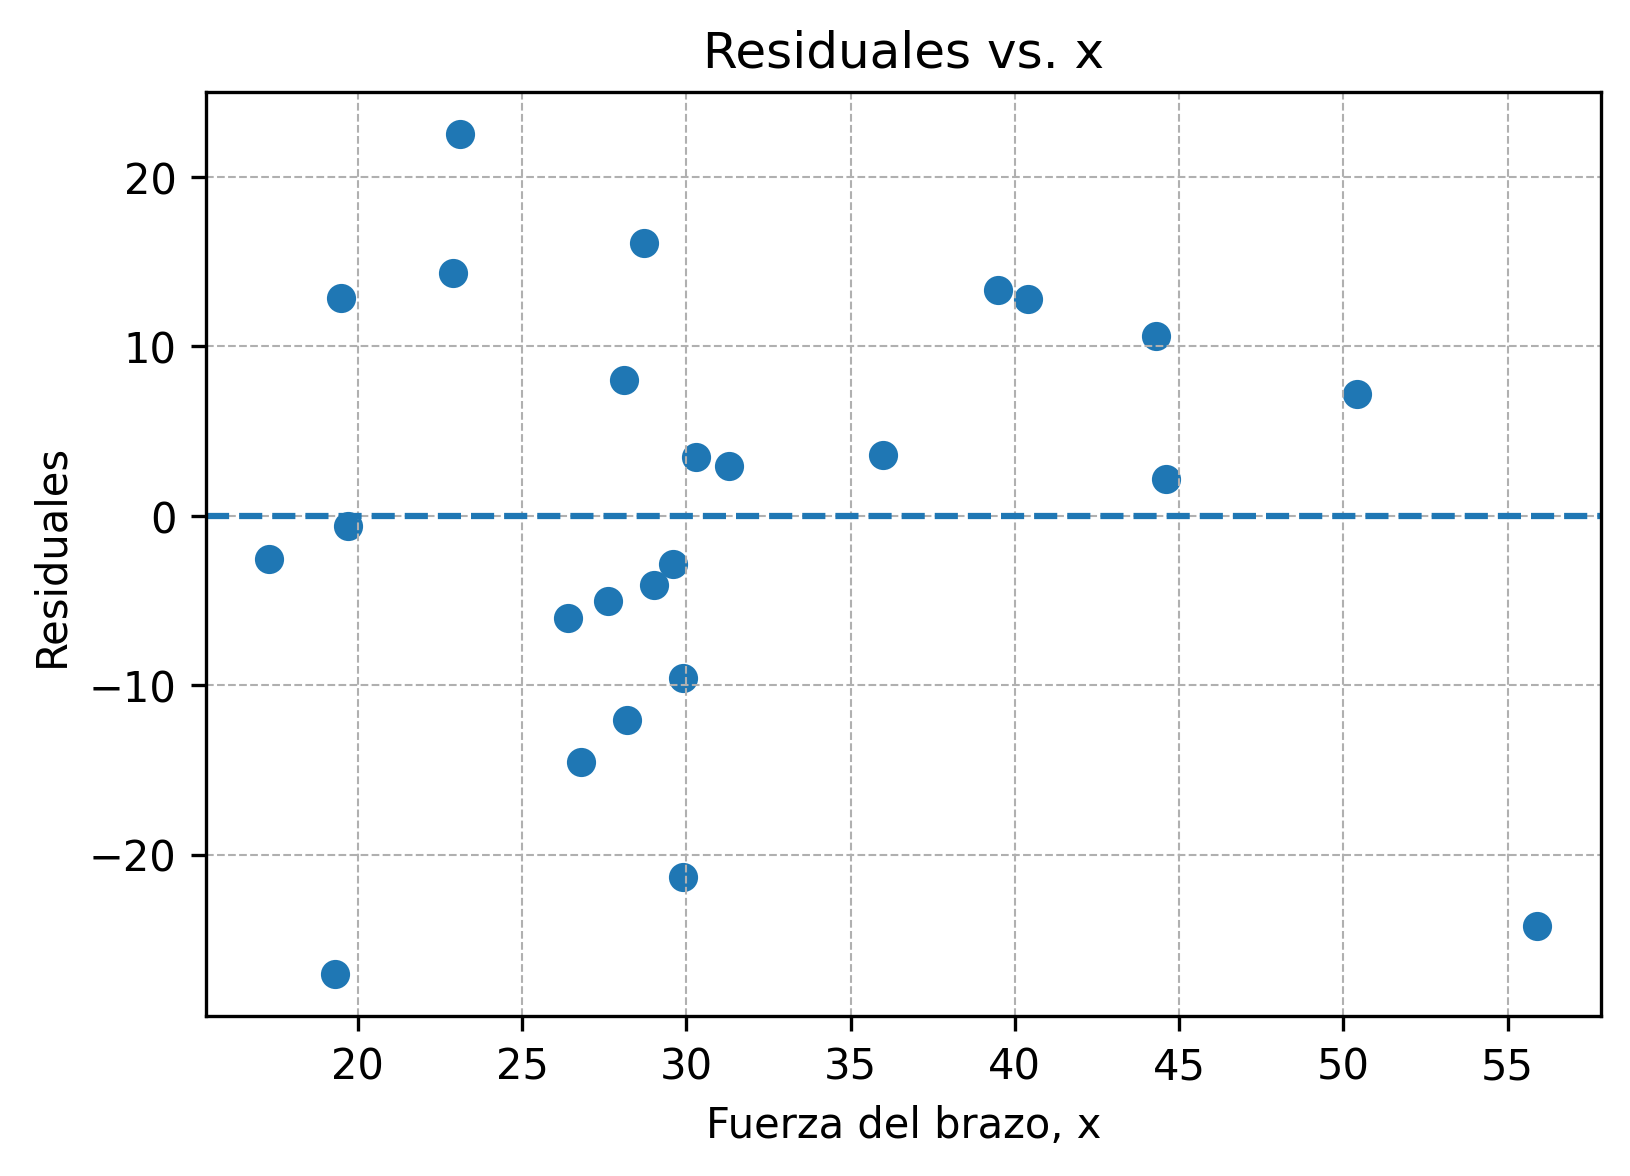
\includegraphics[width=0.7\textwidth]{../plots/python/ejercicio1/residuals_plot.png}
				\caption{Residuales vs. $x$.}
				\label{fig:resid}
			\end{figure} 
		}
	\end{itemize}

\section{Ejercicio 2}
Doce marcas de shampoo de venta en México han compartido información
acerca de sus ventas y del monto en inversión publicitaria durante 2023. Los
datos anuales de ambas variables se presentan a continuación:

\begin{table}[H]
    \centering
    \caption{Ventas y Inversión Publicitaria en Redes Sociales (2023)}
    \label{tab:shampoo_datos}
    \begin{tabular}{|c|c|c|}
        \hline
        \textbf{Marca} & \textbf{Ventas (Millones de lts.)} & \textbf{Inversión (Millones de pesos)} \\
        \hline
        A & 2.4 & 6 \\
        B & 1.6 & 2 \\
        C & 2.3 & 5 \\
        D & 1.5 & 1 \\
        E & 3.2 & 4 \\
        F & 2.5 & 7 \\
        G & 1.8 & 4 \\
        H & 1.8 & 3 \\
        I & 3.5 & 8 \\
        J & 3.4 & 11 \\
        K & 1.5 & 2 \\
        L & 3.2 & 12 \\
        \hline
    \end{tabular}
\end{table}

\begin{itemize}
    \item \textbf{a.} Realice el diagrama de dispersión entre las variables, obtenga e interpreta las estadísticas descriptivas de las mismas.\\
\textcolor{blue}{
El diagrama de dispersión de la Figura~\ref{fig:sh_scatter} sugiere una relación positiva clara entre inversión en redes ($x$) y ventas ($y$).
\begin{figure}[H]
    \centering
    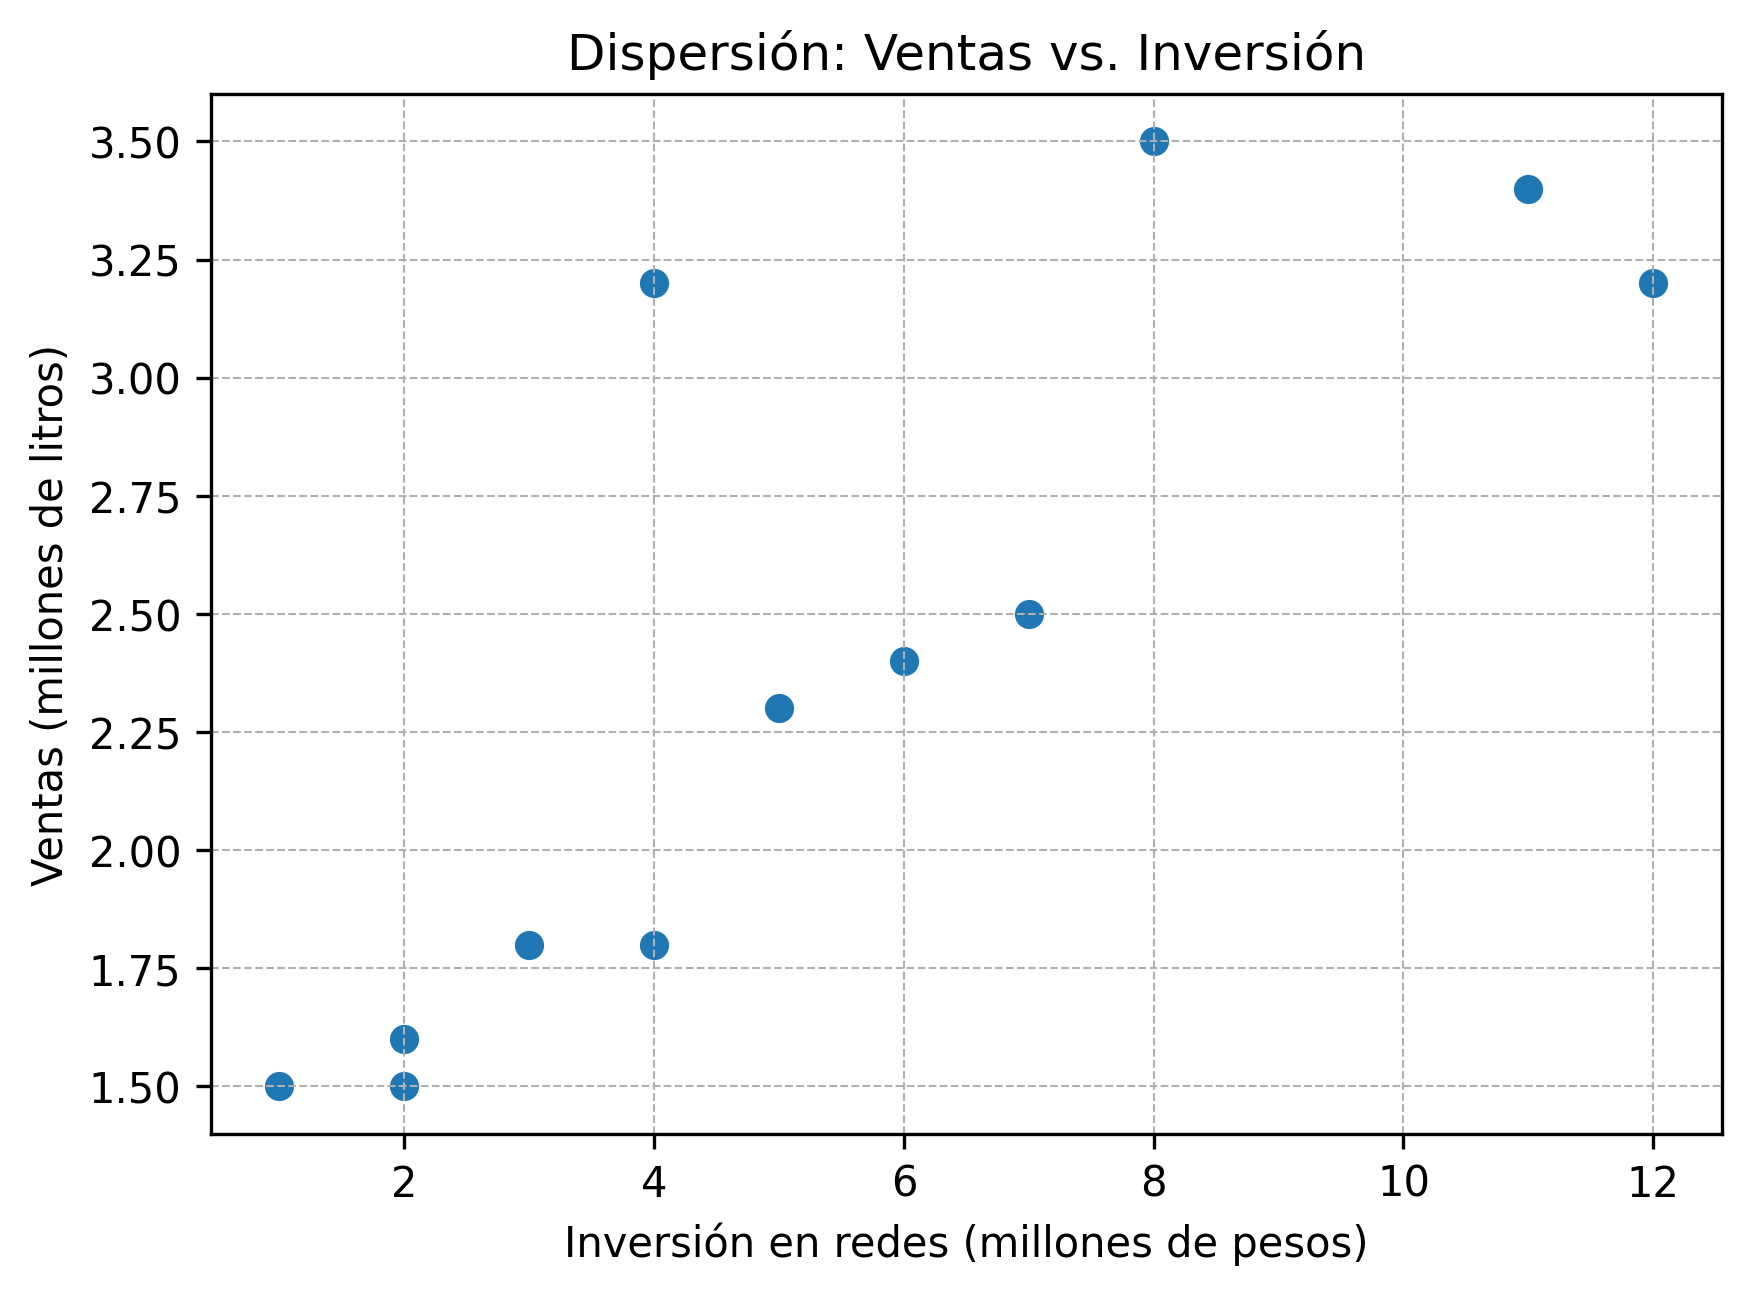
\includegraphics[width=0.70\textwidth]{../plots/python/ejercicio2/scatter_plot.png}
    \caption{Dispersión: Ventas vs. Inversión en redes.}
    \label{fig:sh_scatter}
\end{figure}
\noindent\textbf{Estadísticas descriptivas}
\begin{center}
\begin{tabular}{lccccccc}
\hline
Variable & Media & Mediana & Desv. Est. & Min & Q1 & Q3 & Max \\
\hline
Ventas $y$ (mill. lts.) & 2.392 & 2.35 & 0.768 & 1.50 & 1.75 & 3.20 & 3.50 \\
Inversión $x$ (mill. pesos) & 5.417 & 4.50 & 3.528 & 1.00 & 2.75 & 7.25 & 12.00 \\
\hline
\end{tabular}
\end{center}
}

    \item \textbf{b.} Calcule el intervalo de confianza al 95\% para coeficiente de correlación lineal.\\
\textcolor{blue}{
Se obtuvo el coeficiente de Pearson
\[ r = 0.8334, \qquad p\text{-valor} = 0.000759. \]
Vía la transformación $z$ de Fisher, el intervalo de confianza al 95\% es
\[ \big[\,0.4974,\;0.9520\,\big]. \]
Como $p<0.05$ y el IC no incluye 0, existe evidencia de una relación lineal positiva entre $x$ e $y$.
}

    \item \textbf{c.} Estime los coeficientes del modelo de regresión lineal simple por MCO.\\
\textcolor{blue}{
El modelo estimado es
\[ \hat{y} = 1.4089 + 0.1814\,x, \qquad R^2 = 0.695. \]
La pendiente es estadísticamente significativa ($t=4.769$, $p=0.001$). La Figura~\ref{fig:sh_line} muestra la recta ajustada.
\begin{figure}[H]
    \centering
    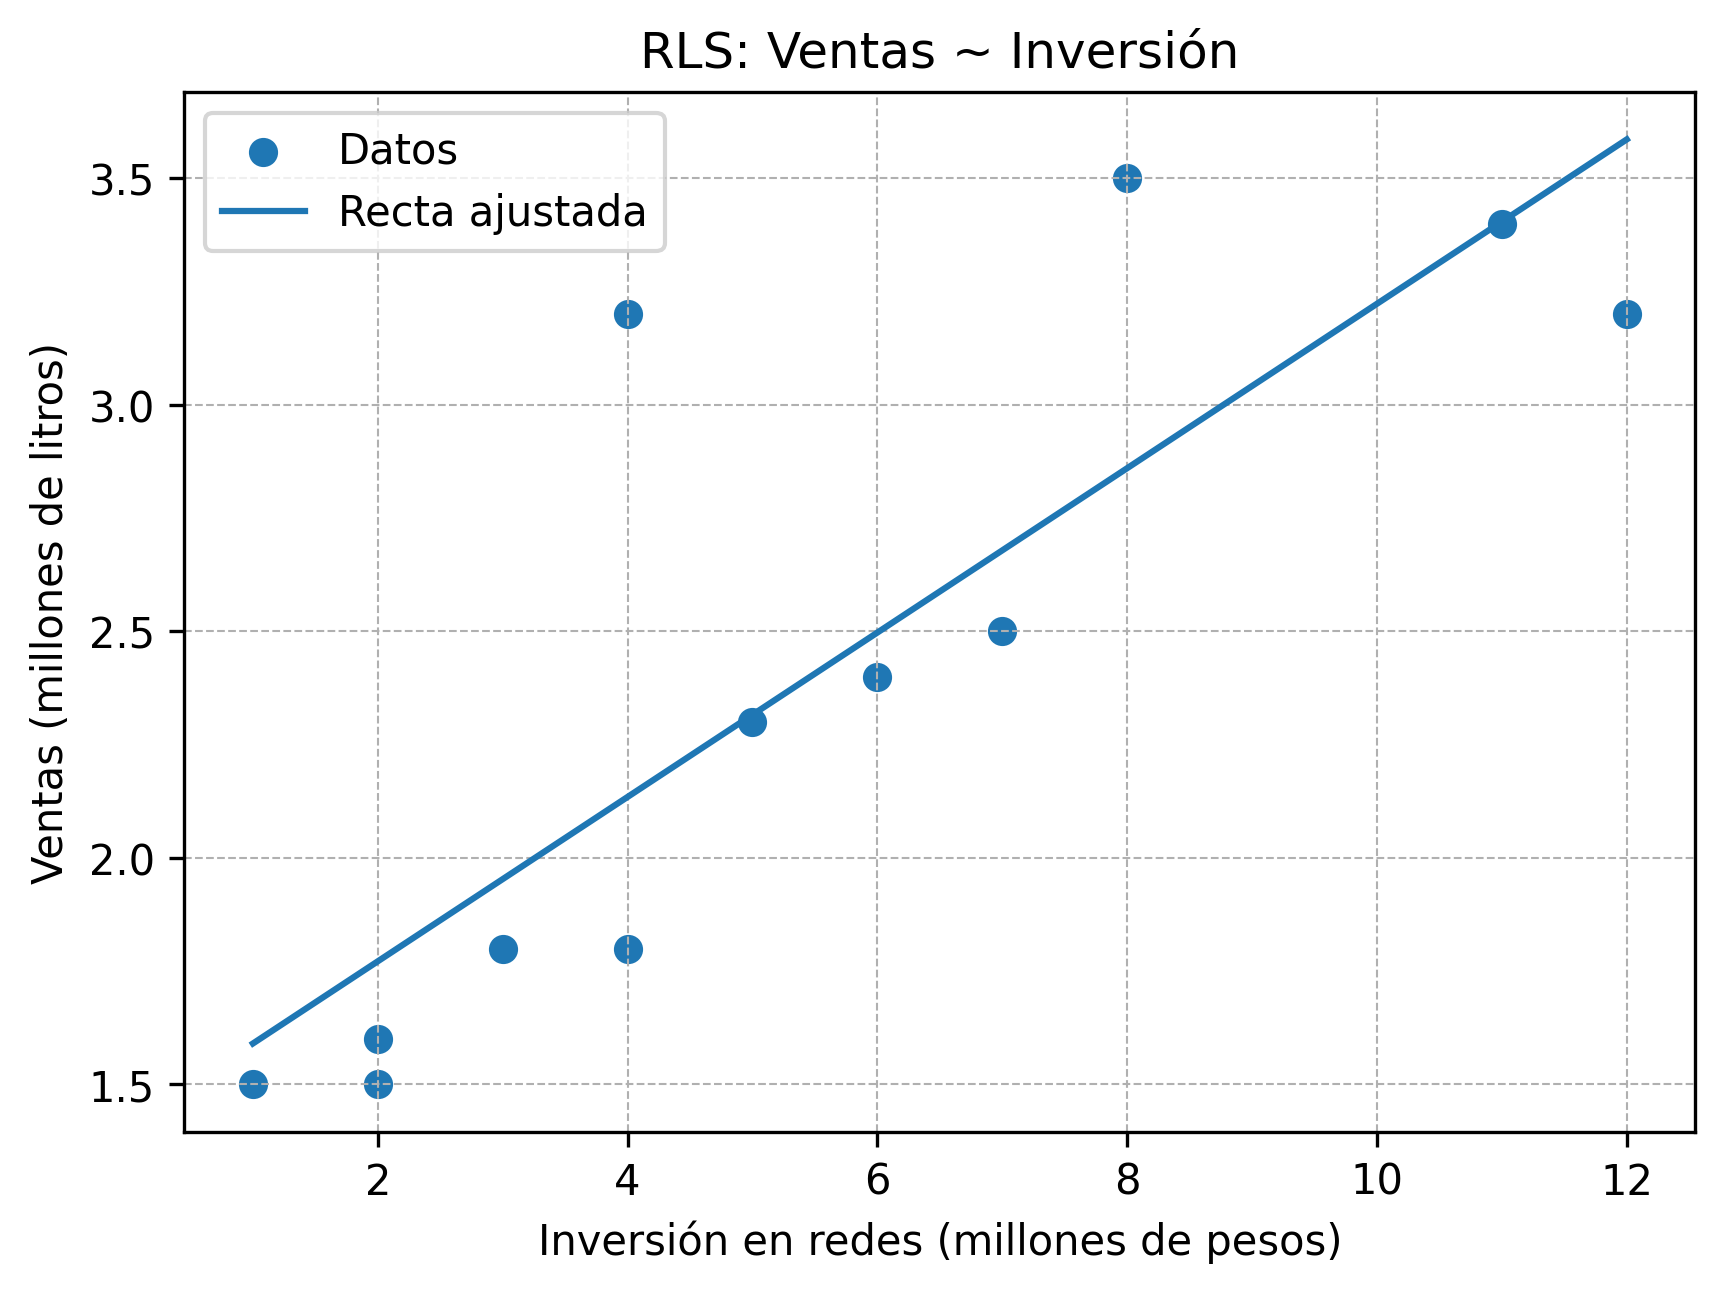
\includegraphics[width=0.72\textwidth]{../plots/python/ejercicio2/shampoo_rls_line.png}
    \caption{RLS: Ventas (mill. lts.) en función de Inversión en redes (mill. pesos).}
    \label{fig:sh_line}
\end{figure}
}

    \item \textbf{d.} Utilizando un nivel de significancia del 5\%, pruebe la hipótesis estadística de que por cada 500 mil pesos adicionales de inversión anual en redes sociales, se espera un incremento en las ventas anuales de shampoo mayor a 50 mil litros.\\
\textcolor{blue}{
Formulamos $H_0: \beta_1 \le 0.1$ vs. $H_1: \beta_1 > 0.1$, donde $\beta_1$ se mide en millones de litros por millón de pesos. Con $\hat{\beta}_1=0.1814$, $SE(\hat{\beta}_1)=0.0380$, $df=10$:
\[ t = \frac{\hat{\beta}_1 - 0.1}{SE(\hat{\beta}_1)} = 2.1404, \qquad p\text{-valor}=0.0290. \]
Como $p<0.05$, \textbf{se rechaza $H_0$}. En unidades del enunciado, por $0.5$ millones de pesos el incremento esperado es
\[ 0.1814\times 0.5 = 0.0907 \text{ millones de litros } (= 90.7\,\text{mil lts.}) > 50\,\text{mil lts.} \]
}
\end{itemize}

\section{Ejercicio 3}
El siguiente juego de datos describe la producción de esencia floral en una comunidad en Francia. La variable independiente ($X$) se refiere a la cantidad de flores procesadas para extraer su esencia por cada productor (en miles de unidades). La variable dependiente ($Y$) es una medida del aceite extraído en onzas por la cantidad de flores procesadas.

\begin{table}[H]
    \centering
    \caption{Datos de flores procesadas ($X$) y producción de esencia ($Y$)}
    \label{tab:flowers}
    \begin{tabular}{|c|c|c|}
        \hline
        \textbf{Obs.} & \textbf{Flores $X$ (miles)} & \textbf{Producción $Y$ (onzas)} \\
        \hline
        1  & 1.00 & 1.71 \\
        2  & 1.08 & 1.52 \\
        3  & 1.15 & 1.29 \\
        4  & 1.15 & 3.09 \\
        5  & 1.20 & 2.21 \\
        6  & 1.30 & 2.26 \\
        7  & 1.37 & 2.40 \\
        8  & 1.37 & 2.10 \\
        9  & 1.43 & 1.96 \\
        10 & 1.46 & 2.09 \\
        11 & 1.52 & 2.02 \\
        12 & 1.57 & 1.31 \\
        13 & 1.65 & 2.17 \\
        14 & 1.65 & 2.28 \\
        15 & 1.65 & 2.41 \\
        16 & 1.66 & 2.23 \\
        17 & 1.87 & 3.04 \\
        18 & 2.03 & 2.06 \\
        19 & 2.05 & 2.73 \\
        20 & 2.30 & 2.36 \\
        \hline
    \end{tabular}
\end{table}

\begin{itemize}
    \item \textbf{a.} Grafique los datos en un diagrama de dispersión.\\
\textcolor{blue}{
La Figura~\ref{fig:fl_scatter} muestra el diagrama de dispersión entre flores procesadas ($x$) y producción de esencia ($y$). Se observa una tendencia positiva tenue.\\
\begin{figure}[H]
    \centering
    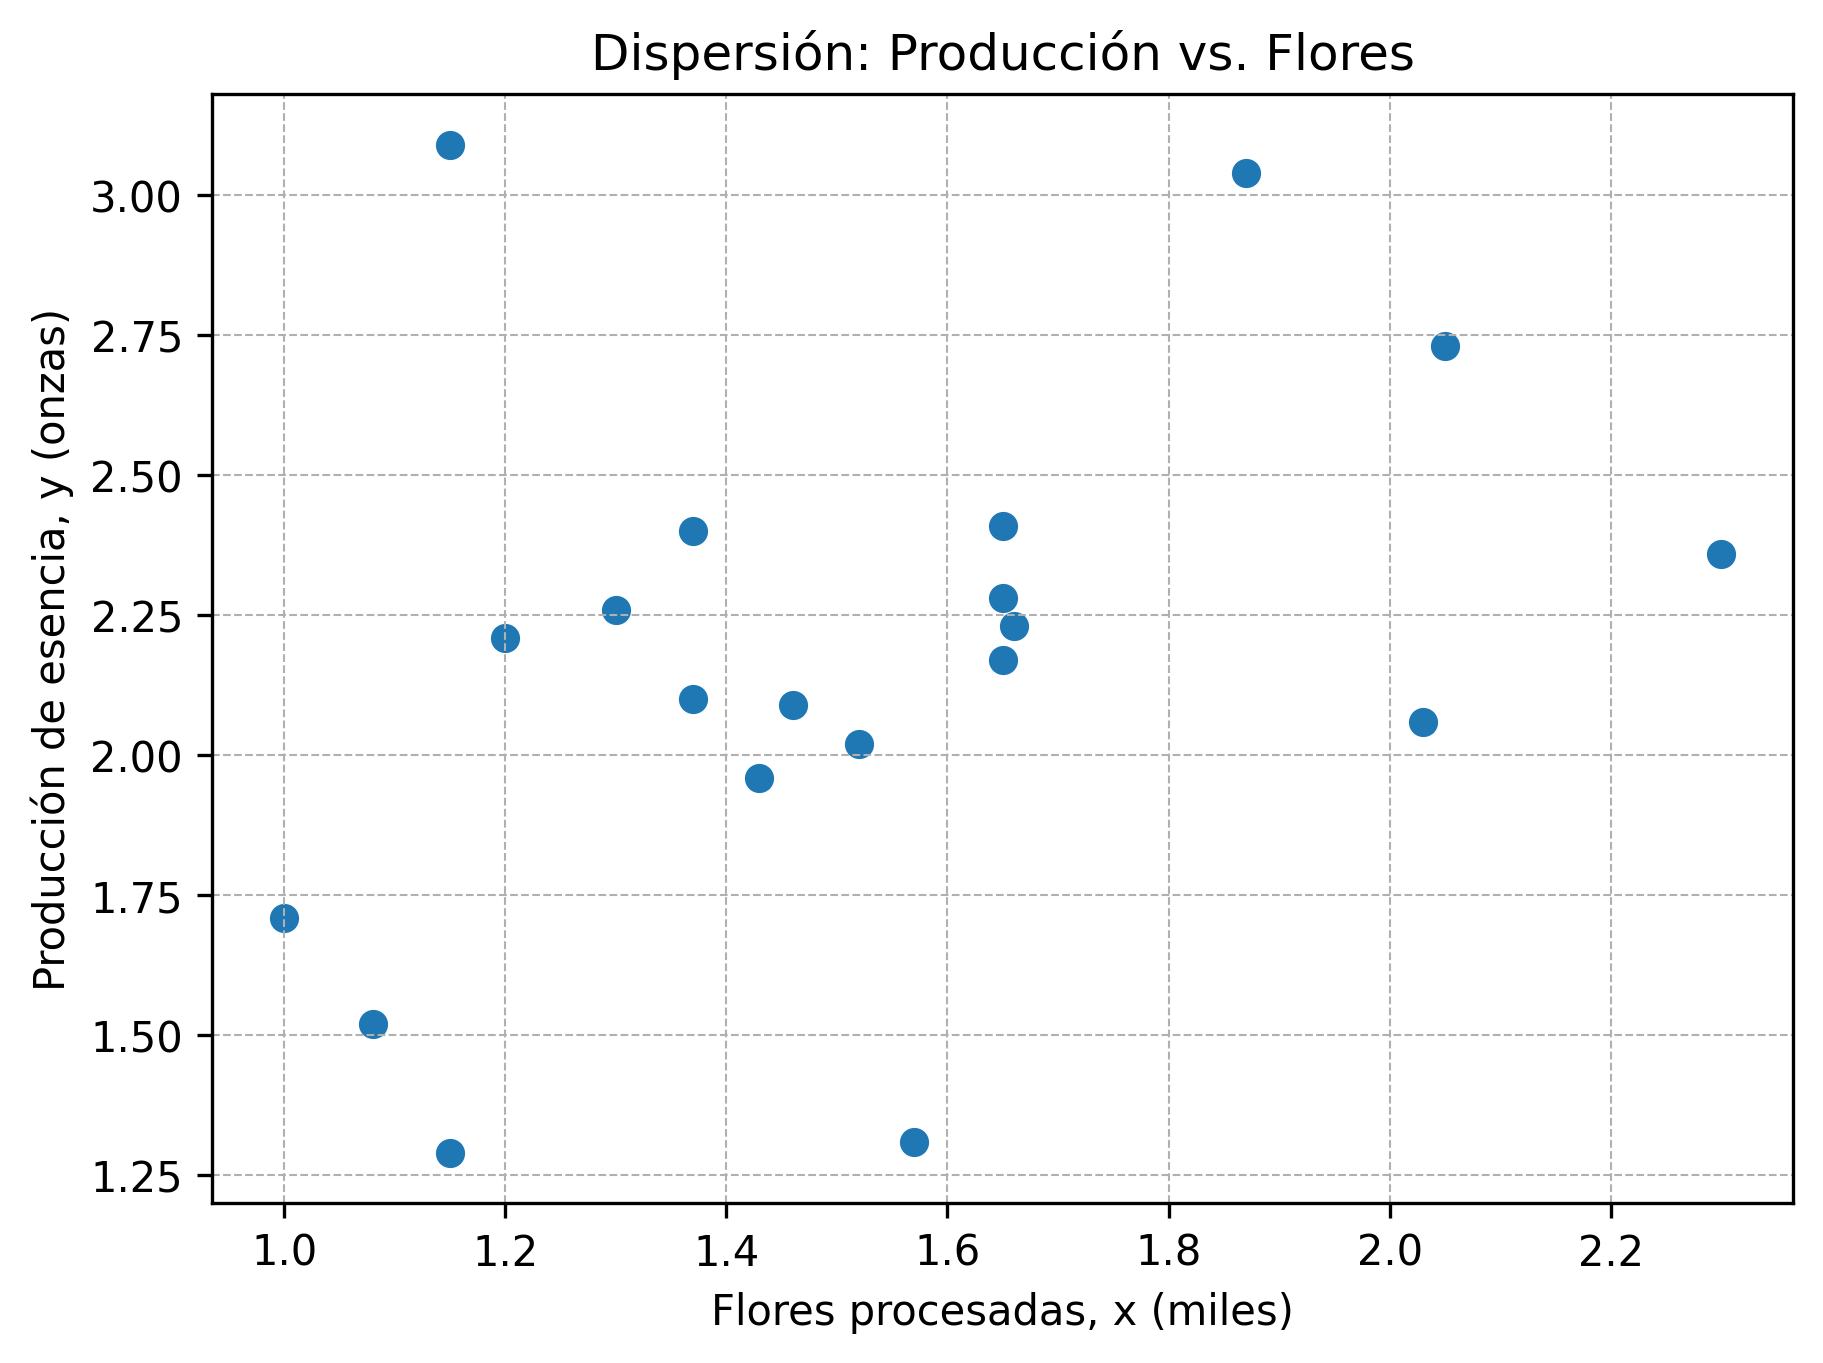
\includegraphics[width=0.72\textwidth]{../plots/python/ejercicio3/scatter_flowers.png}
    \caption{Dispersión: Producción vs. Flores.}
    \label{fig:fl_scatter}
\end{figure}
\noindent\textbf{Estadísticas descriptivas }
\begin{center}
\begin{tabular}{lccccccc}
\hline
Variable & Media & Mediana & Desv. Est. & Min & Q1 & Q3 & Max \\
\hline
$x$ (flores, miles) & 1.523 & 1.49 & 0.347 & 1.00 & 1.275 & 1.652 & 2.30 \\
$y$ (producción, onzas) & 2.162 & 2.19 & 0.477 & 1.29 & 2.005 & 2.370 & 3.09 \\
\hline
\end{tabular}
\end{center}
}

    \item \textbf{b.} ¿Cree que exista una relación entre la producción de esencia y la cantidad de flores procesadas? ¿Es esta positiva o negativa?\\
\textcolor{blue}{
El coeficiente de Pearson fue
\[ r = 0.3757, \qquad p\text{-valor} = 0.1026, \qquad IC_{95\%}(r) = [-0.0802,\;0.7016]. \]
La relación estimada es \emph{positiva}, pero la evidencia al 5\% no es concluyente (el $p$-valor es mayor que $0.05$ y el IC incluye 0).
}

    \item \textbf{c.} Por medio del ajuste de una línea recta, verifique que: $b_0 = 1.38$, $b_1 = 0.52$, $S^2 = 0.206$.\\
\textcolor{blue}{
Mediante MCO se obtuvo
\[ \hat{y} = 1.3756 + 0.5163\,x, \qquad S^2 = \frac{\mathrm{SSE}}{n-2} = 0.2064. \]
Estos valores coinciden con los de referencia (diferencias $<\!0.005$). La Figura~\ref{fig:fl_line} muestra la recta ajustada.
\begin{figure}[H]
    \centering
    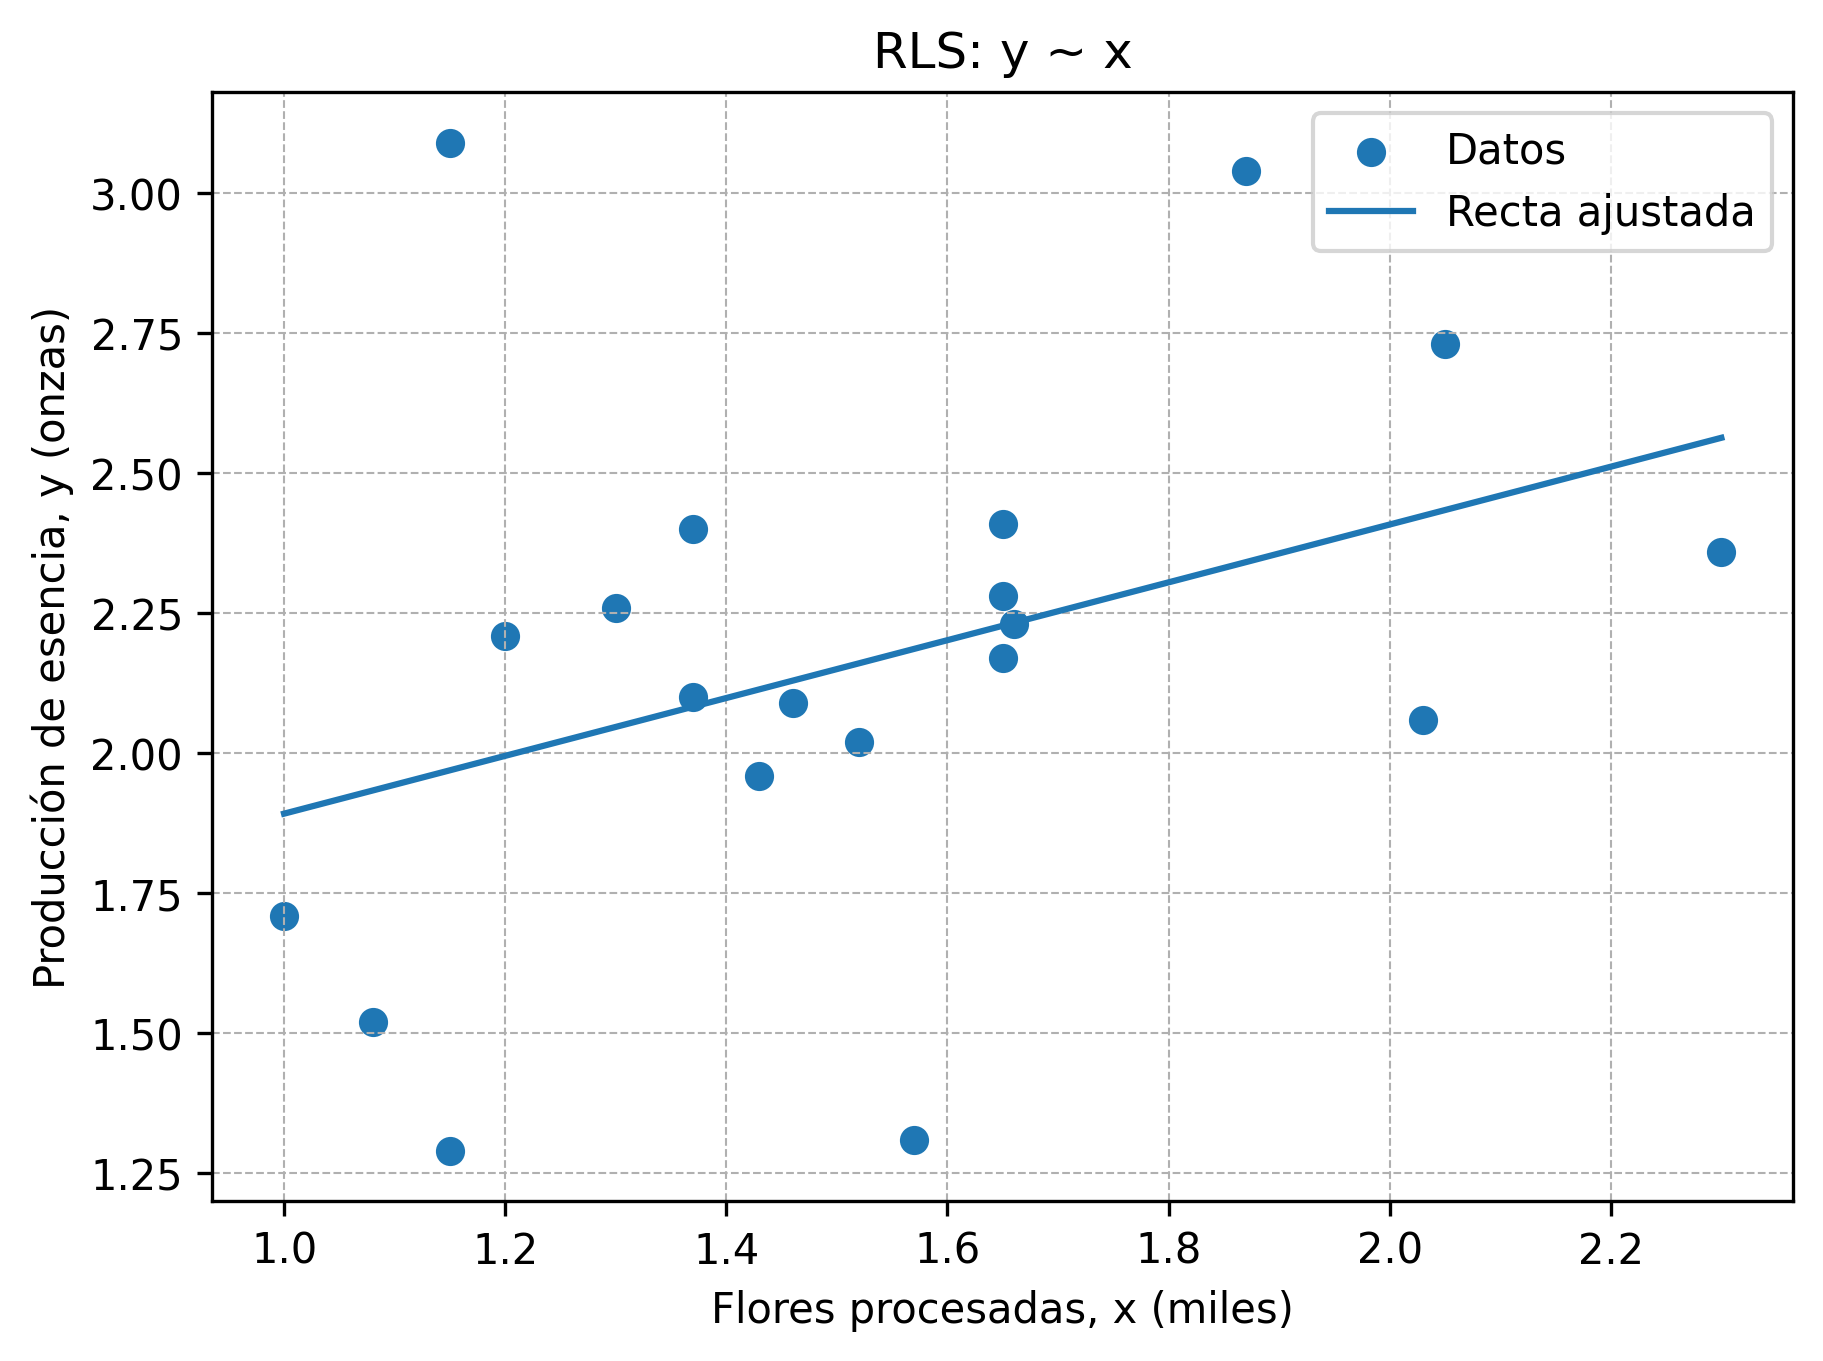
\includegraphics[width=0.78\textwidth]{../plots/python/ejercicio3/rls_line.png}
    \caption{RLS: $y$ en función de $x$.}
    \label{fig:fl_line}
\end{figure}
}

\item \textbf{d.} Construya la tabla de análisis de varianza (ANOVA) y realice la prueba de significancia para la regresión. ¿Es esta significativa o no?\\
	\begingroup
	\color{blue}

	Con $n=20$ observaciones: 
	\[
	\mathrm{SSR}=0.6104,\; \mathrm{SSE}=3.7153,\; \mathrm{SST}=4.3257,
	\quad R^2=\frac{\mathrm{SSR}}{\mathrm{SST}}=0.1411.
	\]

	\begin{table}[H]
	\centering
	\captionsetup{labelfont={color=blue}, textfont={color=blue}}
	\arrayrulecolor{blue}
	{\color{blue}
	\caption{ANOVA }
	\label{tab:anova_ej3}
	\begin{tabular}{|l|r|r|r|}
		\hline
		\textbf{Fuente} & \textbf{SC} & \textbf{gl} & \textbf{CM} \\
		\hline
		Regresión & 0.6104 & 1  & 0.610435 \\
		Error     & 3.7153 & 18 & 0.206405 \\
		Total     & 4.3257 & 19 & --       \\
		\hline
	\end{tabular}
	}
	\end{table}

La prueba $F$ da
\[
  F=\frac{\mathrm{MSR}}{\mathrm{MSE}}=\frac{0.6104/1}{3.7153/18}=2.9575,
  \qquad p=0.1026.
\]
Conclusión: a un 5\% de significancia, \emph{no} es significativa (no se rechaza $H_0$).

\endgroup

    \item \textbf{e.} Encuentre el error estándar de la pendiente y un intervalo de confianza al 95\%.\\
\textcolor{blue}{
\[ \mathrm{SE}(\hat{\beta}_1) = 0.3002, \qquad IC_{95\%}(\beta_1) = [-0.1144,\;1.1471]. \]
La pendiente no es significativa al 5\% porque el IC incluye 0.
}

    \item \textbf{f.} ¿Qué porcentaje de la variabilidad total de la respuesta es explicado por el modelo? (Sugerencia: bondad de ajuste).\\
\textcolor{blue}{
\[ R^2 = 0.1411 \;\Rightarrow\; 14.11\% \text{ de la variabilidad de } y \text{ es explicada por } x. \]
}

    \item \textbf{g.} Determine un intervalo de confianza para la respuesta media al 95\% cuando el número de flores procesadas es igual a $x=1.25$.\\
\textcolor{blue}{
Para $x_0=1.25$:
\[ \widehat{E[y\mid x_0]} = 2.0210, \qquad IC_{95\%}:\; [\,1.7468,\; 2.2953\,]. \]
}

    \item \textbf{h.} Determine un intervalo de predicción al 95\% cuando el número de flores procesadas es igual a $x=1.95$.\\
\textcolor{blue}{
Para $x_0=1.95$:
\[ \hat{y}(x_0) = 2.3825, \qquad \text{PI}_{95\%}:\; [\,1.3680,\; 3.3969\,]. \]
}
\end{itemize}

\section{Ejercicio 4- Usando Dataset de la tarea anterior}
Considere el ejemplo de servicio de TV por cable descrito a continuación.

\subsection*{Encuesta de televisión por cable}
Una empresa de televisión por cable encargó a un bufete un estudio de mercado para conocer el perfil de los clientes potenciales de una zona residencial formada por dos colonias. Las colonias constan de 12 y 25 manzanas con un total de 236 y 605 hogares, respectivamente. Mediante muestreo probabilístico (no discutido aquí) se seleccionó una muestra de ocho manzanas y cinco hogares por manzana. En cada hogar seleccionado se recabaron varias respuestas de las que presentamos solamente algunas de éstas.


\begin{table}[H]
    \centering
    \arrayrulecolor{black}
    \caption{Tabla 2: Encuesta de televisión por cable}
    \label{tab:cable_vars}
    \begin{tabular}{|p{2.8cm}|p{10.5cm}|}
        \hline
        \textbf{Variable} & \textbf{Descripción} \\
        \hline
        1. Colonia & Colonia a la que pertenece el hogar de la zona residencial \\
        \hline
        2. Manzana & Número de manzana a la que pertenece el hogar \\
        \hline
        3. Adultos & Número de adultos por hogar \\
        \hline
        4. Niños & Número de niños menores de 12 años por hogar \\
        \hline
        5. Teles & Número de televisores por hogar \\
        \hline
        6. Tipo & Tipo de televisor que posee: blanco y negro (B), color (C), ambos (A) \\
        \hline
        7. Tvtot & Suma del número de horas frente al televisor en la semana de todos los miembros de la familia \\
        \hline
        8. Renta & Cantidad máxima de renta que el jefe del hogar estaría dispuesto a pagar al mes por servicio de TV por cable (múltiplos de \$5) \\
        \hline
        9. Valor & Valor catastral del hogar (m\$). La respuesta se usa para dar idea aproximada del ingreso familiar \\
        \hline
    \end{tabular}
\end{table}

% Tabla con los datos muestrales cableTV.xlsx
\begin{table}[H]
    \centering
    \caption{Datos muestrales: hogares (n=40)}
    \label{tab:cable_data}
    \scriptsize
    \resizebox{\textwidth}{!}{%
    \begin{tabular}{|r|r|r|r|r|r|r|r|c|r|}
        \hline
        \textbf{Obs.} & \textbf{Colonia} & \textbf{Manzana} & \textbf{Adultos} & \textbf{Niños} & \textbf{Teles} & \textbf{Renta} & \textbf{TVtot} & \textbf{Tipo} & \textbf{Valor} \\
        \hline
        1 & 2 & 20 & 3 & 2 & 2 & 50 & 68 & B & 79928 \\
        2 & 2 & 25 & 3 & 3 & 1 & 65 & 82 & B & 94415 \\
        3 & 2 & 20 & 1 & 2 & 1 & 45 & 40 & A & 120896 \\
        4 & 2 & 8 & 2 & 2 & 2 & 35 & 56 & A & 132867 \\
        5 & 2 & 25 & 1 & 2 & 0 & 0 & 0 & N & 141901 \\
        6 & 2 & 14 & 1 & 2 & 0 & 0 & 0 & N & 147997 \\
        7 & 2 & 22 & 2 & 1 & 1 & 65 & 30 & A & 156410 \\
        8 & 2 & 20 & 3 & 1 & 3 & 45 & 62 & C & 156841 \\
        9 & 2 & 25 & 3 & 3 & 2 & 70 & 82 & A & 157041 \\
        10 & 2 & 20 & 2 & 2 & 3 & 45 & 60 & C & 161222 \\
        11 & 2 & 8 & 3 & 2 & 1 & 70 & 84 & A & 162509 \\
        12 & 2 & 8 & 2 & 1 & 3 & 45 & 34 & A & 180124 \\
        13 & 2 & 14 & 2 & 1 & 1 & 55 & 38 & C & 180437 \\
        14 & 2 & 8 & 2 & 1 & 2 & 45 & 42 & A & 190314 \\
        15 & 2 & 14 & 2 & 3 & 1 & 55 & 86 & A & 192265 \\
        16 & 2 & 25 & 1 & 2 & 3 & 70 & 40 & B & 192816 \\
        17 & 2 & 14 & 4 & 2 & 4 & 75 & 84 & C & 193279 \\
        18 & 2 & 20 & 4 & 3 & 3 & 55 & 14 & C & 205656 \\
        19 & 1 & 2 & 3 & 1 & 3 & 50 & 31 & C & 216190 \\
        20 & 2 & 22 & 1 & 1 & 3 & 65 & 42 & C & 216321 \\
        21 & 2 & 22 & 4 & 2 & 2 & 75 & 76 & C & 216465 \\
        22 & 2 & 22 & 2 & 3 & 2 & 40 & 74 & C & 225694 \\
        23 & 1 & 4 & 3 & 1 & 3 & 60 & 35 & C & 237752 \\
        24 & 2 & 25 & 1 & 1 & 1 & 55 & 22 & C & 241531 \\
        25 & 2 & 8 & 1 & 3 & 2 & 75 & 54 & C & 249098 \\
        26 & 1 & 9 & 2 & 1 & 3 & 65 & 27 & C & 252221 \\
        27 & 1 & 9 & 3 & 1 & 4 & 65 & 35 & C & 261763 \\
        28 & 2 & 14 & 2 & 2 & 1 & 65 & 52 & C & 269898 \\
        29 & 2 & 22 & 2 & 3 & 4 & 60 & 70 & C & 271556 \\
        30 & 1 & 2 & 3 & 3 & 3 & 65 & 69 & C & 279163 \\
        31 & 1 & 4 & 3 & 2 & 3 & 60 & 54 & C & 299558 \\
        32 & 1 & 9 & 4 & 0 & 4 & 70 & 32 & B & 311195 \\
        33 & 1 & 4 & 2 & 0 & 4 & 75 & 16 & C & 318551 \\
        34 & 1 & 2 & 3 & 0 & 4 & 70 & 24 & A & 322652 \\
        35 & 1 & 4 & 2 & 0 & 2 & 60 & 20 & C & 329198 \\
        36 & 1 & 2 & 2 & 0 & 2 & 60 & 20 & A & 332699 \\
        37 & 1 & 2 & 3 & 0 & 3 & 70 & 28 & C & 336290 \\
        38 & 1 & 9 & 3 & 0 & 5 & 85 & 28 & C & 355641 \\
        39 & 1 & 9 & 2 & 0 & 3 & 70 & 20 & C & 357972 \\
        40 & 1 & 4 & 3 & 0 & 4 & 80 & 28 & C & 370325 \\
        \hline
    \end{tabular}%
    }
\end{table}

\begin{itemize}
    \item \textbf{a.} Ajuste por mínimos cuadrados un modelo de regresión lineal simple para la respuesta \textbf{Renta}, con el \textbf{Valor} catastral (en miles de pesos) como variable independiente. Calcule los coeficientes y el error estándar de la regresión, y grafique los residuales contra el regresor $x$ (gráfica de dispersión).\\
    \begingroup\color{blue}
    Con todos los datos, el modelo estimado por MCO es
    \[
      \widehat{\text{Renta}} = \hat\beta_0 + \hat\beta_1 x,\quad \hat\beta_0=30.3232,\; \hat\beta_1=0.1225.
    \]
    El error estándar de la regresión es \(\sigma = \sqrt{\mathrm{MSE}} = 15.2446\).

    \begin{figure}[H]
      \centering
      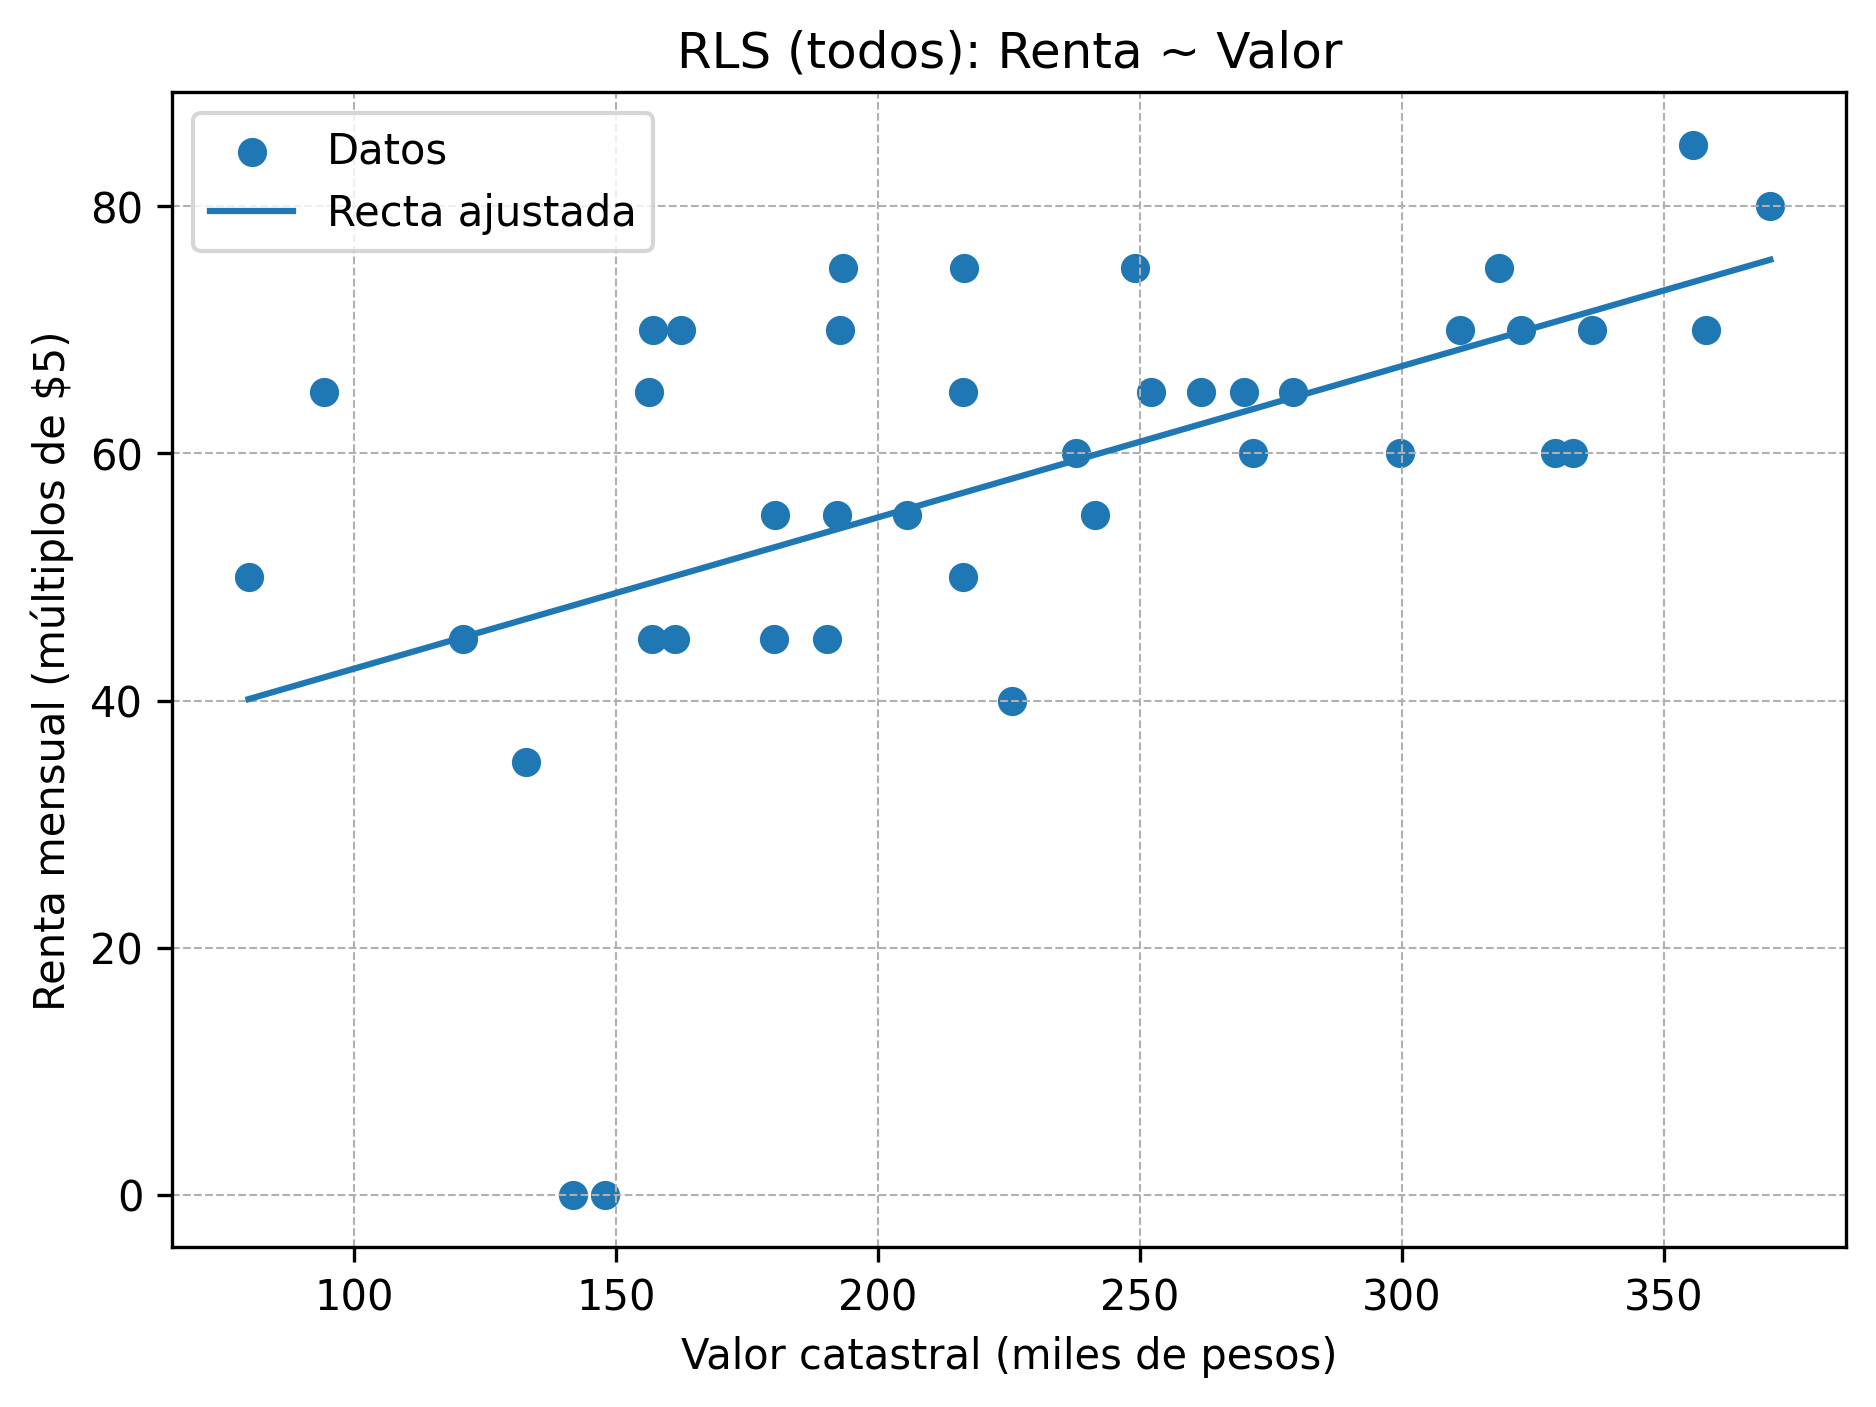
\includegraphics[width=0.75\textwidth]{../plots/python/ejercicio4/full_scatter_line.png}
      \caption{RLS (todos): Renta vs. Valor catastral.}
      \label{fig:cable_full_line}
    \end{figure}
    \begin{figure}[H]
      \centering
      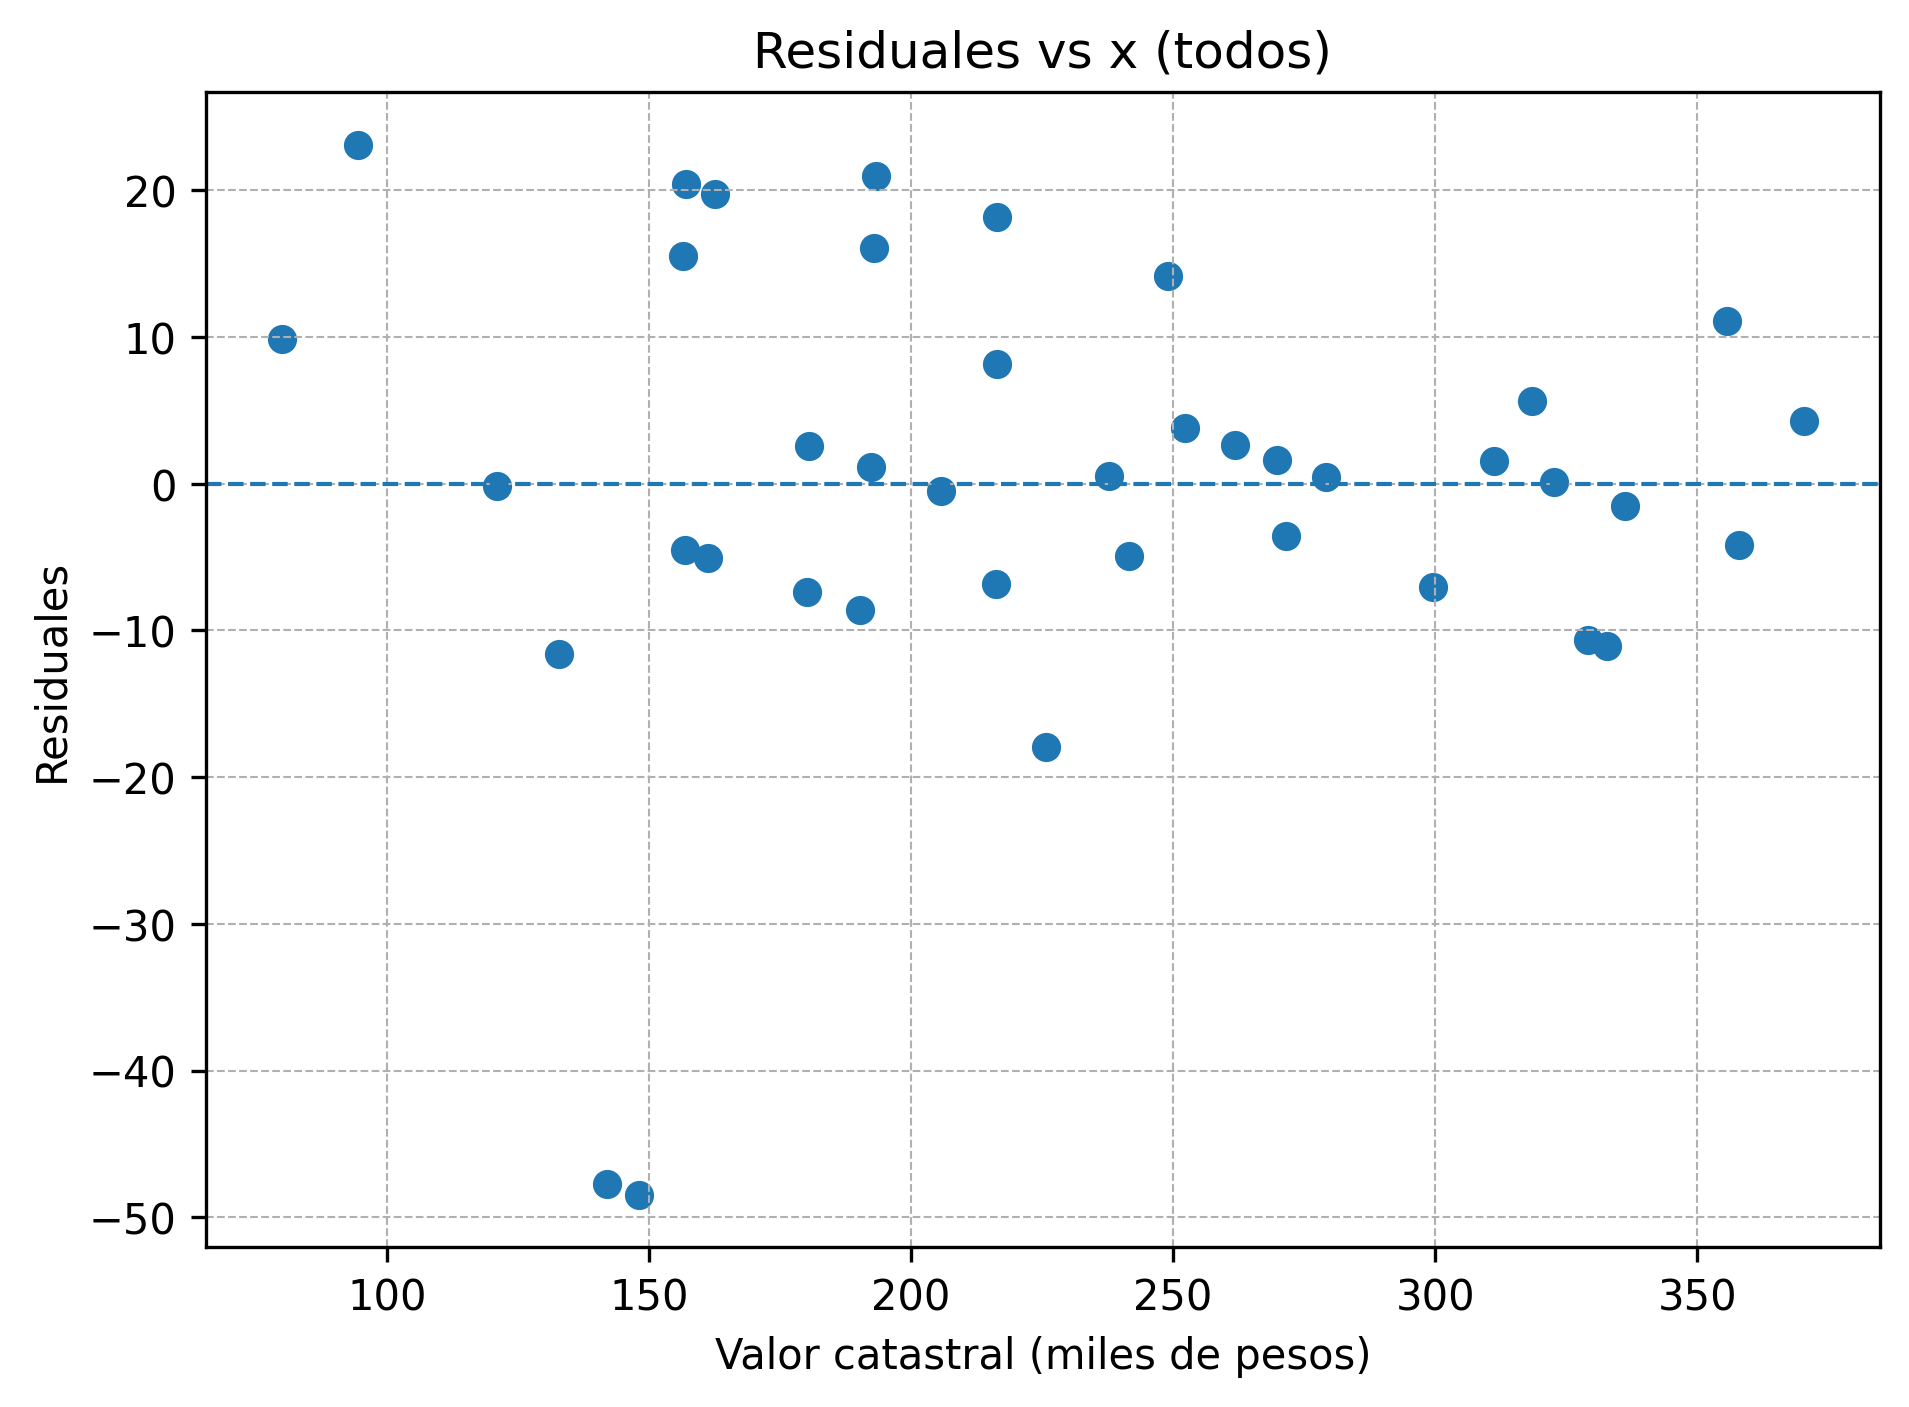
\includegraphics[width=0.75\textwidth]{../plots/python/ejercicio4/full_resid_vs_x.png}
      \caption{Residuales vs. $x$ (todos).}
      \label{fig:cable_full_resid}
    \end{figure}
    \endgroup
    \item \textbf{b.} ¿Cuál es la significancia de la regresión? (valor-$p$ del estadístico $F$).\\
    \begingroup\color{blue}
    Para todos los datos, la ANOVA de la regresión produce:
    \begin{table}[H]
      \centering
      \captionsetup{labelfont={color=blue}, textfont={color=blue}}
      \arrayrulecolor{blue}
      {\color{blue}
      \caption{ANOVA (todos los datos)}
      \label{tab:cable_anova_full}
      \begin{tabular}{|l|r|r|r|r|r|}
        \hline
        \textbf{Fuente} & \textbf{gl} & \textbf{SC} & \textbf{CM} & \textbf{$F$} & \textbf{$p$} \\
        \hline
        Regresión & 1  & 3496.3622 & 3496.3622 & 15.0447 & 0.000404 \\
        Error     & 38 & 8831.1378 &  232.3984 &   --     &   --     \\
        Total     & 39 & 12327.5000 &      --    &   --     &   --     \\
        \hline
      \end{tabular}}
    \end{table}
    Por tanto,
    \[
      F=15.0447,\qquad p=0.000404,\qquad R^2=0.2836.
    \]
    Conclusión: la regresión es \emph{significativa} al 5\% (se rechaza $H_0: \beta_1=0$).
    \endgroup
    \item \textbf{c.} Repita los incisos anteriores pero sin considerar los 2 casos donde $y=0$. ¿Consideraría los nuevos coeficientes estadísticamente iguales a los anteriores? Comente.\\
    \begingroup\color{blue}
    Excluyendo los dos casos con $y=0$, el modelo es
    \[
      \widehat{\text{Renta}} = \hat\beta_0 + \hat\beta_1 x,\quad \hat\beta_0=41.7885,\; \hat\beta_1=0.0840,\quad \sigma=10.0569.
    \]
    \begin{figure}[H]
      \centering
      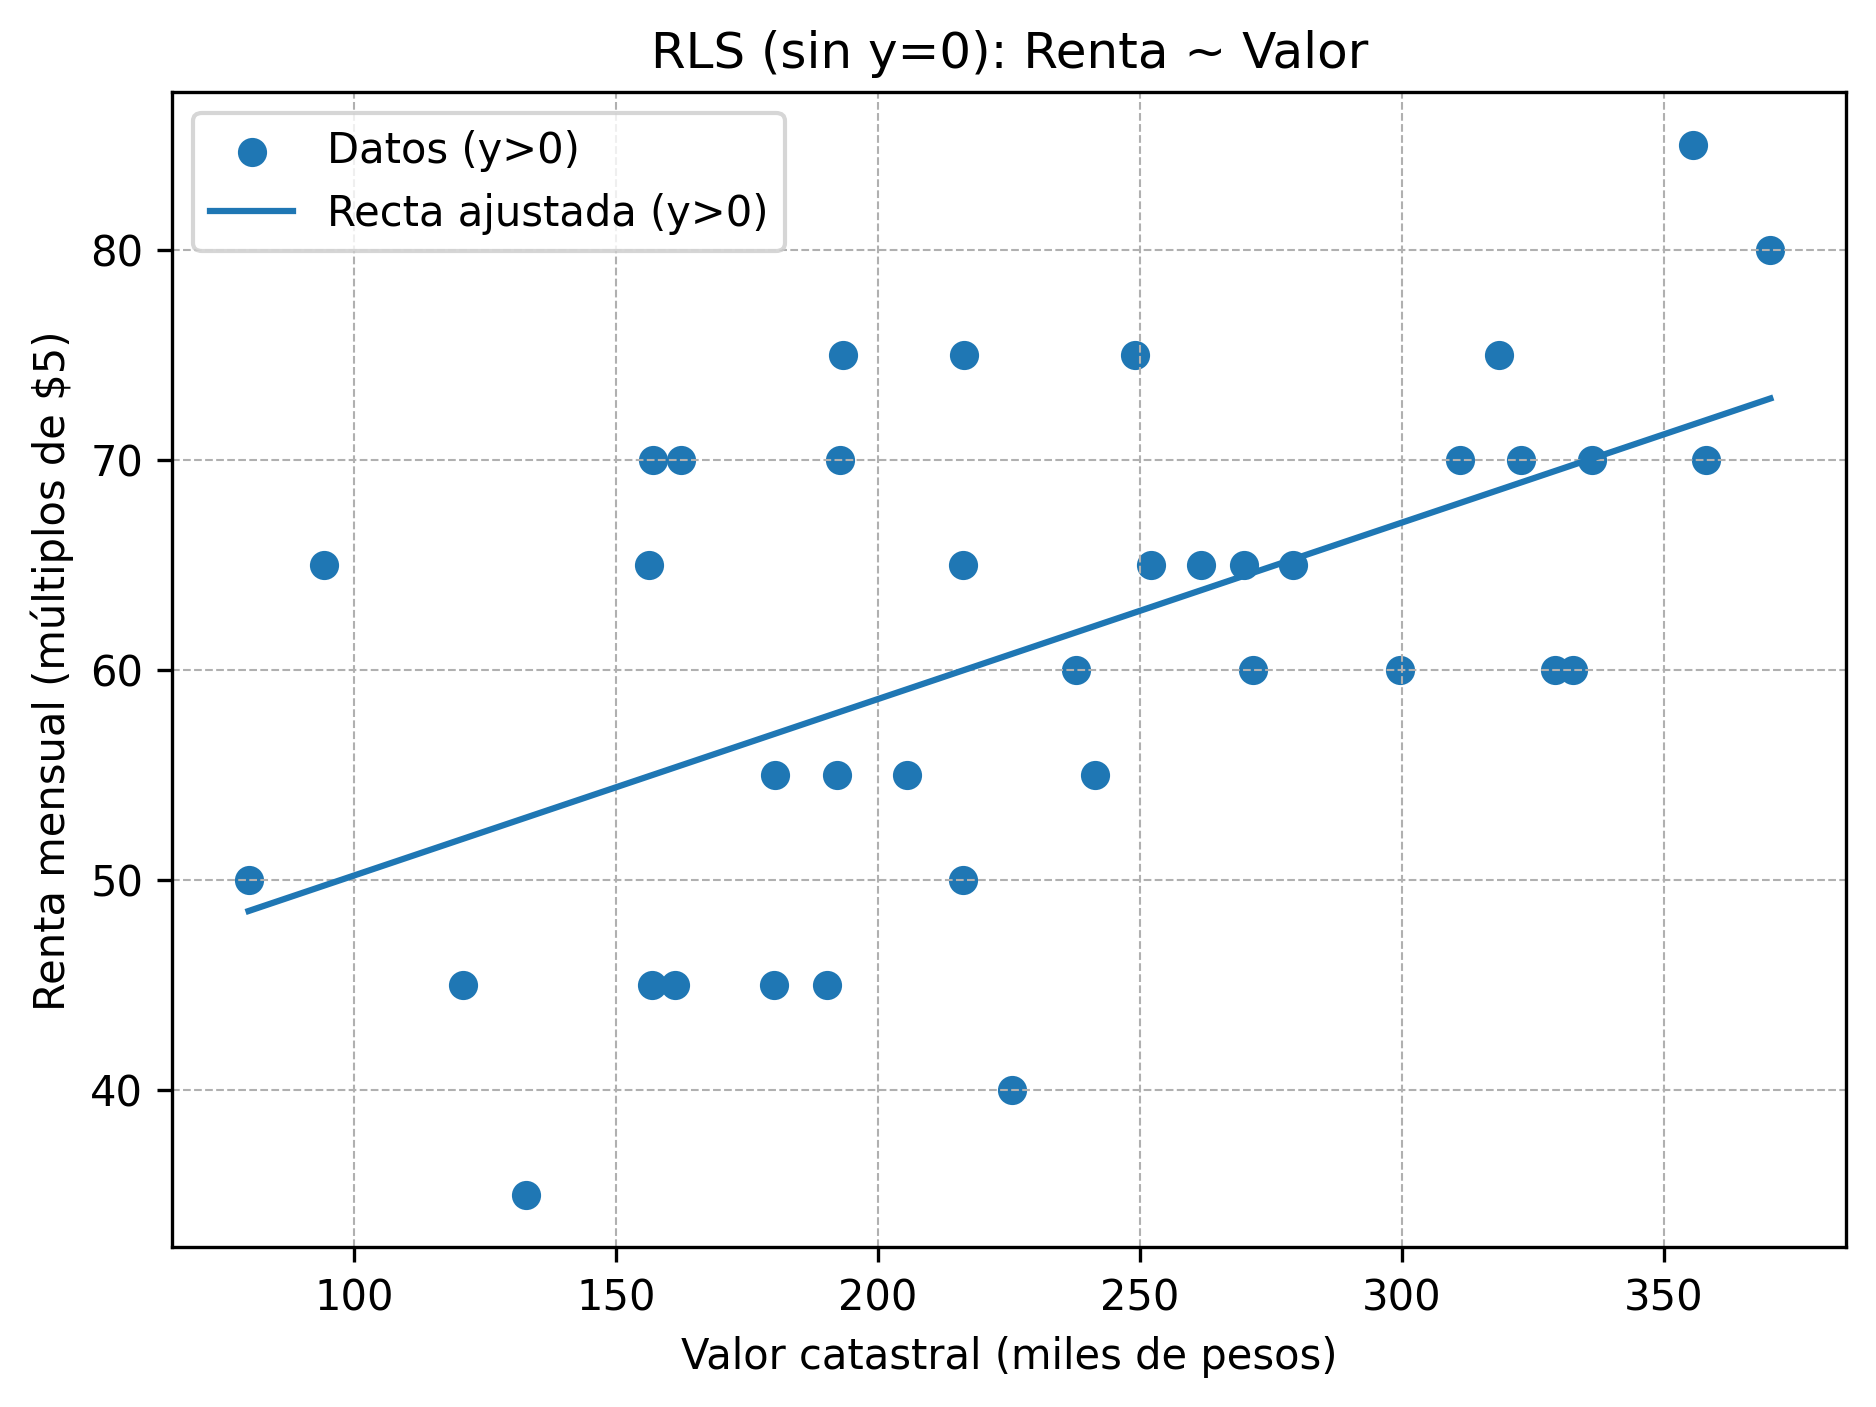
\includegraphics[width=0.75\textwidth]{../plots/python/ejercicio4/nz_scatter_line.png}
      \caption{RLS (sin $y=0$): Renta vs. Valor catastral.}
      \label{fig:cable_nz_line}
    \end{figure}
    \begin{figure}[H]
      \centering
      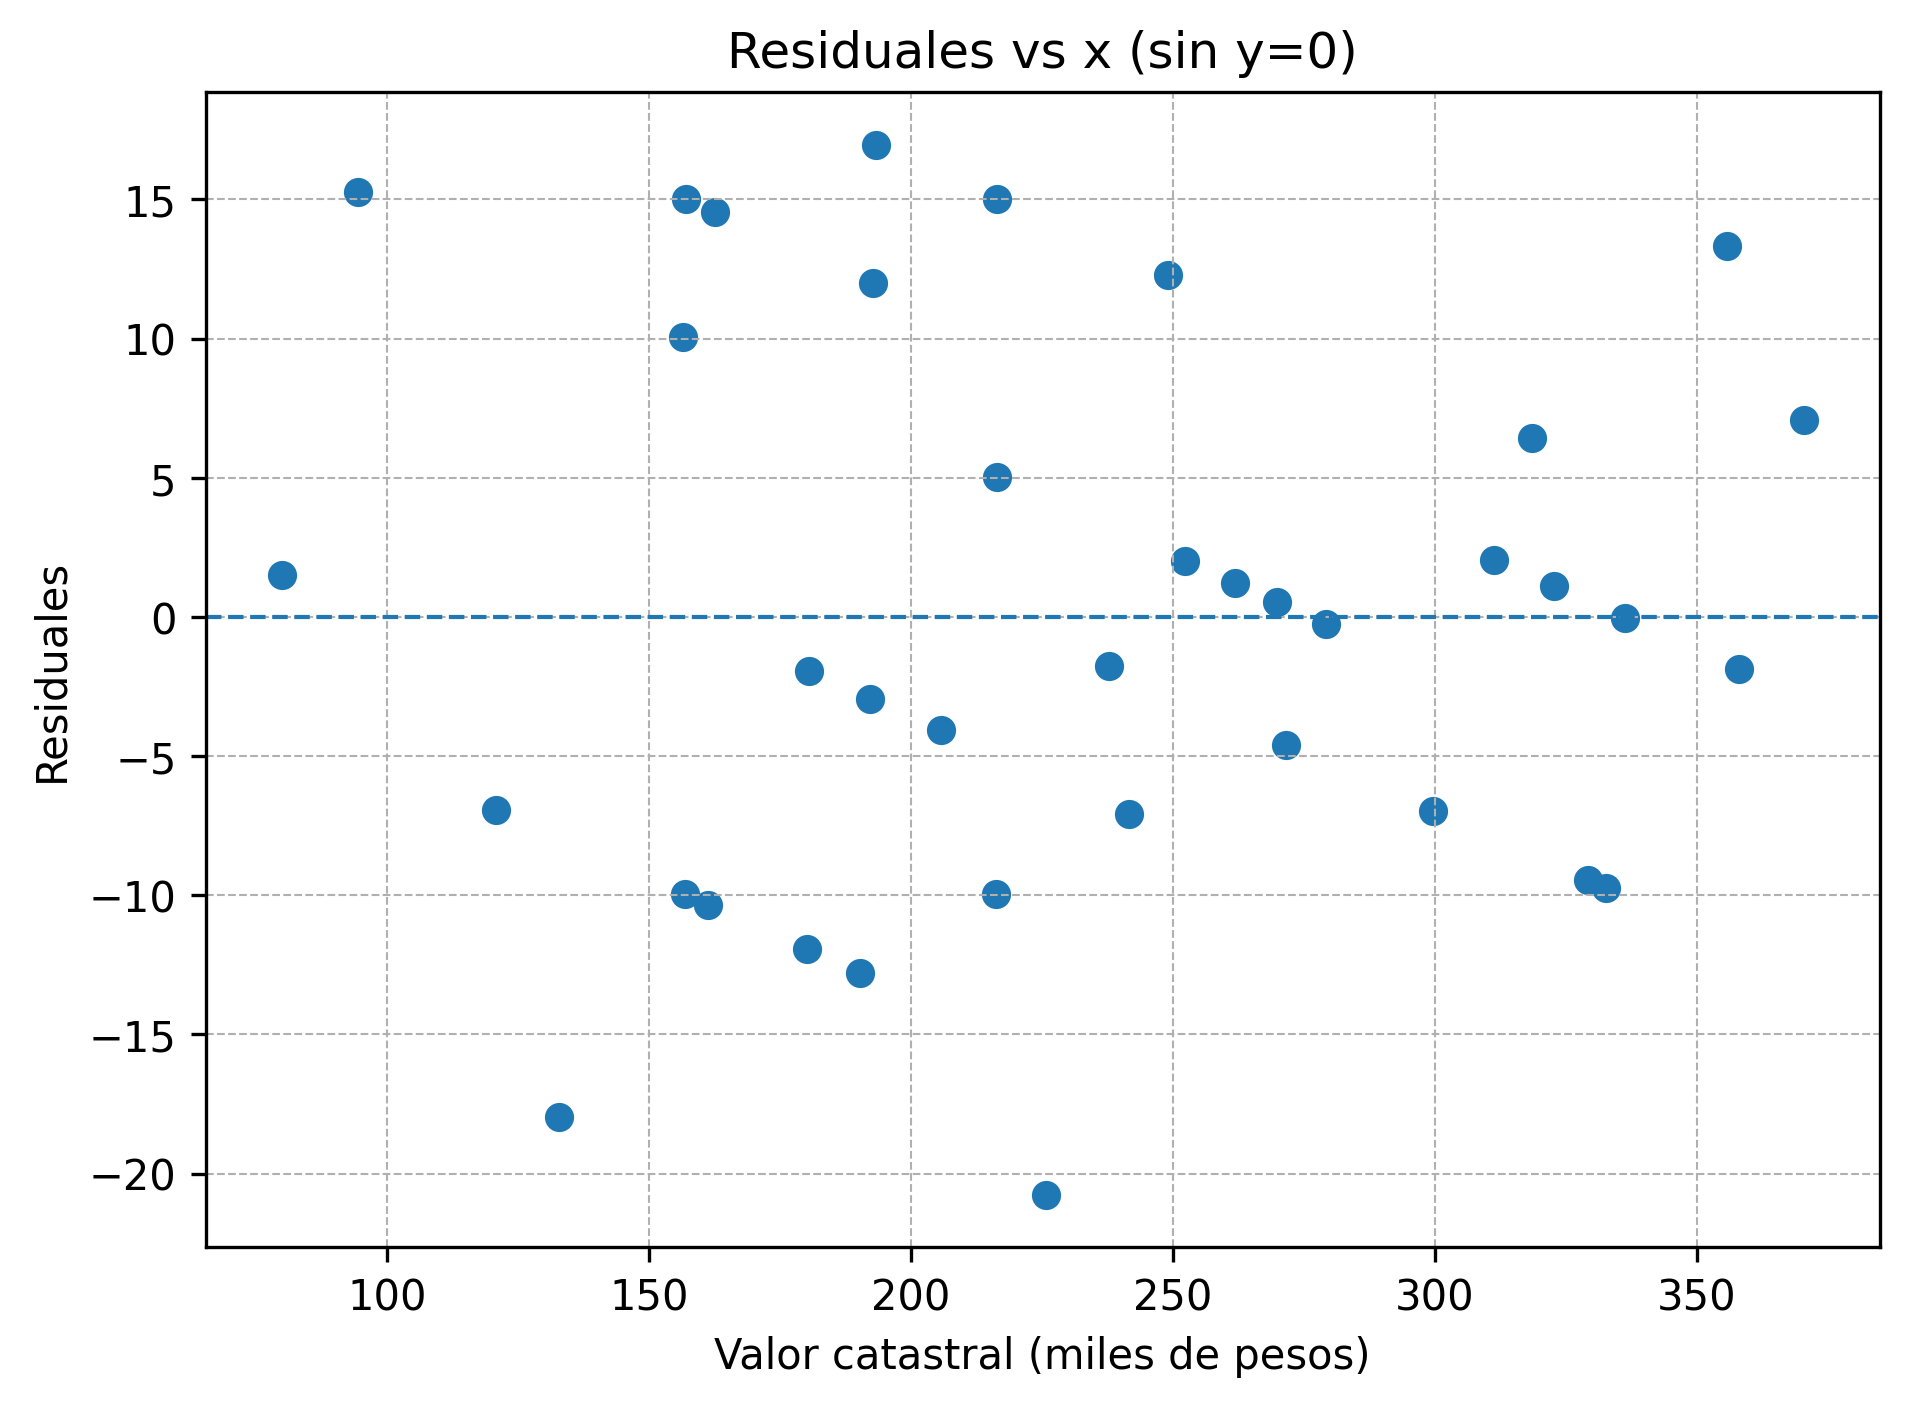
\includegraphics[width=0.75\textwidth]{../plots/python/ejercicio4/nz_resid_vs_x.png}
      \caption{Residuales vs. $x$ (sin $y=0$).}
      \label{fig:cable_nz_resid}
    \end{figure}

    \noindent ANOVA (sin $y=0$):
    \begin{table}[H]
      \centering
      \captionsetup{labelfont={color=blue}, textfont={color=blue}}
      \arrayrulecolor{blue}
      {\color{blue}
      \caption{ANOVA (sin $y=0$)}
      \label{tab:cable_anova_nz}
      \begin{tabular}{|l|r|r|r|r|r|}
        \hline
        \textbf{Fuente} & \textbf{gl} & \textbf{SC} & \textbf{CM} & \textbf{$F$} & \textbf{$p$} \\
        \hline
        Regresión & 1  & 1543.1332 & 1543.1332 & 15.2572 & 0.000396 \\
        Error     & 36 & 3641.0773 &  101.1410 &   --     &   --     \\
        Total     & 37 & 5184.2105 &      --    &   --     &   --     \\
        \hline
      \end{tabular}}
    \end{table}
    Los coeficientes cambian (intercepto mayor y pendiente menor), pero ambos modelos muestran pendiente positiva significativa ($p<0.001$).
    \endgroup
    \item \textbf{d.} Compare los coeficientes de determinación $R^2$ en ambos casos. Comente.\\
    \begingroup\color{blue}
    \begin{table}[H]
      \centering
      \captionsetup{labelfont={color=blue}, textfont={color=blue}}
      \arrayrulecolor{blue}
      {\color{blue}
      \caption{Comparativo de ajuste}
      \label{tab:cable_comp}
      \begin{tabular}{|l|r|r|r|r|}
        \hline
        \textbf{Modelo} & $\hat\beta_0$ & $\hat\beta_1$ & $R^2$ & $\sigma$ \\
        \hline
        Todos los datos   & 30.3232 & 0.1225 & 0.2836 & 15.2446 \\
        Sin $y=0$        & 41.7885 & 0.0840 & 0.2977 & 10.0569 \\
        \hline
      \end{tabular}}
    \end{table}
    Se observa una leve mejora en \(R^2\) al remover los dos ceros: 
    \[ R^2_{\text{todos}}=0.2836, \qquad R^2_{\text{sin }y=0}=0.2977. \]
    Esto sugiere que los ceros podrían corresponder a hogares sin disposición de pago (no-demanda) y afectan el ajuste lineal.
    \endgroup
\end{itemize}

\section{Ejercicio 5}
Determine cuáles de entre los siguientes modelos son lineales en los parámetros, en las variables, o en ambos. ¿Cuáles de estos modelos son modelos de regresión lineal?

\begin{enumerate}
  \item[(a)] $Y_i \,=\, \beta_0 \, + \, \beta_1\,\dfrac{1}{X_i} \, + \, \varepsilon_i$\\ \textcolor{blue}{Es lineal en los parámetros $(\beta_0,\beta_1)$ porque puede escribirse como $\beta_0+\beta_1 z_i$ con $z_i=1/X_i$. No es lineal en la variable original $X_i$ (sí lo es en $z_i$). \textbf{Sí es un modelo de regresión lineal} (RLS) usando $1/X_i$ como regresor.}
  \item[(b)] $Y_i \,=\, \beta_0 \, + \, \beta_1\,\ln X_i \, + \, \varepsilon_i$\\ \textcolor{blue}{Lineal en los parámetros; no lineal en $X_i$ pero lineal en el regresor transformado $\ln X_i$. \textbf{Sí es RLS} con $\ln X_i$ como variable explicativa.}
  \item[(c)] $Y_i \,=\, \beta_0\, X_i^{\beta_1} \, + \, \varepsilon_i$\\ \textcolor{blue}{\emph{No lineal en los parámetros} (porque $\beta_1$ está en el exponente) ni en $X_i$. Tomar logaritmos da $\ln Y_i = \ln(\beta_0 X_i^{\beta_1} + \varepsilon_i)$, lo cual \textbf{no} equivale a un modelo lineal con error aditivo. Por tanto, \textbf{no es un modelo de regresión lineal} tal como está especificado.}
  \item[(d)] $\ln Y_i \,=\, \beta_0 \, + \, \beta_1\, X_i \, + \, \varepsilon_i$\\ \textcolor{blue}{Lineal en los parámetros y lineal en el regresor $X_i$. \textbf{Sí es RLS}.}
  \item[(e)] $\ln Y_i \,=\, \ln \beta_0 \, + \, \beta_1\,\ln X_i \, + \, \varepsilon_i$\\ \textcolor{blue}{No es lineal en el parámetro $\beta_0$. Reparametrizando $\alpha_0=\ln \beta_0$ se obtiene $\ln Y_i=\alpha_0+\beta_1\ln X_i+\varepsilon_i$, que es lineal en $(\alpha_0,\beta_1)$ y en $\ln X_i$. \textbf{Se puede estimar como RLS}, con restricción implícita $\beta_0>0$ y luego $\beta_0=e^{\alpha_0}$.}
  \item[(f)] $Y_i \,=\, \beta_0 \, + \, \beta_1^{3}\, X_i \, + \, \varepsilon_i$\\ \textcolor{blue}{No es lineal en el parámetro $\beta_1$. Definiendo $\gamma_1=\beta_1^3$ queda $Y_i=\beta_0+\gamma_1 X_i+\varepsilon_i$, lineal en $(\beta_0,\gamma_1)$. \textbf{Se puede estimar como RLS}; luego $\beta_1=\sqrt[3]{\gamma_1}$.}
\end{enumerate}

\section{Link al repositorio con código fuente}
\href{https://github.com/enriquegomeztagle/MCD-Econometria/tree/main/HWs/RLS-Activity}{https://github.com/enriquegomeztagle/MCD-Econometria/tree/main/HWs/RLS-Activity}

\end{document}

%%%%%%
